\documentclass[12pt,a4paper]{article}
\usepackage{graphicx}
\usepackage{amsmath}
\usepackage{siunitx}
\usepackage{geometry}
\usepackage{float}
\usepackage{hyperref}
\geometry{margin=1in}

\title{Rod Cooling Simulation: Convection and Radiation}
\author{Hariton Marian}
\date{\today}

\begin{document}
\maketitle

\begin{abstract}
This report investigates the cooling of a cylindrical rod subjected to convective and radiative heat transfer. Using MATLAB simulations, we compare temperature evolution predicted by convection-only and combined convection+radiation models, and visualize the results using 2D plots and 3D animated cylinders. The study also justifies neglecting internal conduction by evaluating the Biot number for a real material.  
\end{abstract}

\section{Introduction}
The cooling of solid bodies is a classical problem in heat transfer, relevant for electronics, machinery, and thermal management. For slender rods, if the internal thermal resistance is small relative to surface resistance, the lumped capacitance approximation can be applied, allowing the assumption of uniform temperature across the cross-section.

\section{Theory and Derivation}
The starting point is the first law of thermodynamics for a system:
\begin{equation}
dE = \delta Q - \delta L,
\end{equation}
where \(dE\) is the change in total energy, \(\delta Q\) is the heat added, and \(\delta L\) is the work done by the system.

For a rod with negligible motion:
\begin{itemize}
\item No change in kinetic or potential energy: \(dE = dU\)
\item No external work done: \(\delta L = 0\)
\end{itemize}
Thus:
\begin{equation}
dU = \delta Q
\end{equation}

Assuming uniform temperature and constant specific heat:
\begin{equation}
\frac{dU}{dt} = mc \frac{dT}{dt} = \dot Q
\end{equation}
where \(\dot Q\) is the total heat transfer rate, sum of convection and radiation:
\begin{equation}
\dot Q = \dot Q_\text{conv} + \dot Q_\text{rad}
\end{equation}

\subsection{Convection}
Using Newton's law of cooling:
\begin{equation}
\dot Q_\text{conv} = h A_s (T_\infty - T)
\end{equation}

\subsection{Radiation}
Using the Stefan-Boltzmann law:
\begin{equation}
\dot Q_\text{rad} = \epsilon \sigma A_s (T_\infty^4 - T^4)
\end{equation}

Combining these, we obtain the governing ODE:
\begin{equation}
\frac{dT}{dt} = \frac{1}{\rho c V} \left[ h A_s (T_\infty - T) + \epsilon \sigma A_s (T_\infty^4 - T^4) \right]
\end{equation}
where \(V = \pi R^2 L\) and \(A_s = 2\pi R L + 2 \pi R^2\) are the rod volume and surface area, respectively.  

\subsection{Lumped Capacitance Approximation and Biot Number}
The Biot number is defined as
\begin{equation}
\text{Bi} = \frac{h L_c}{k}, \quad L_c = \frac{V}{A_s}
\end{equation}
where \(k\) is the thermal conductivity of the rod material. For a low Biot number (\(\text{Bi} < 0.1\)), the internal temperature gradient is negligible and the lumped capacitance approximation is valid.

\textbf{Example:} Consider an aluminum rod (\(\rho = 2700~\text{kg/m}^3\), \(c = 900~\text{J/kgK}\), \(k = 205~\text{W/mK}\)), length \(L = 0.5~\text{m}\), radius \(R = 0.1~\text{m}\), and convective coefficient \(h = 40~\text{W/m}^2\text{K}\):
\begin{align*}
V &= \pi R^2 L = \pi (0.1)^2 (0.5) \approx 0.0157~\text{m}^3 \\
A_s &= 2\pi R L + 2\pi R^2 = 2\pi(0.1)(0.5) + 2\pi(0.1)^2 \approx 0.345~\text{m}^2 \\
L_c &= \frac{V}{A_s} \approx 0.0455~\text{m} \\
\text{Bi} &= \frac{h L_c}{k} \approx \frac{40 \cdot 0.0455}{205} \approx 0.0089 \ll 0.1
\end{align*}
Hence, internal conduction can be neglected.

\section{Methodology}
\begin{itemize}
\item Parameters (\(\rho, c, L, R, h, \epsilon, T_0, T_\infty\)) were defined.
\item The ODE was integrated numerically using MATLAB \texttt{ode45} with an event function to stop near ambient temperature.
\item An analytical solution for convection-only cooling was used for comparison:
\begin{equation}
T_\text{conv}(t) = T_\infty + (T_0 - T_\infty) \exp(-k_\text{conv} t), \quad k_\text{conv} = \frac{2 h (L+R)}{\rho c L R}
\end{equation}
\item Temperature data were interpolated for smooth 2D and 3D animations.
\item 2D plots show both convection-only and combined convection+radiation curves.
\item 3D cylinders are colored according to instantaneous temperature.
\end{itemize}

\section{Results}
Figure 1 shows the initial simulation with radiation (\(\epsilon = 0.5\)), while Figure 2 shows the case with \(\epsilon = 0\). The two curves overlap almost perfectly, demonstrating that the radiation effect is negligible at small temperature differences for this rod.  

\begin{figure}[H]
\centering
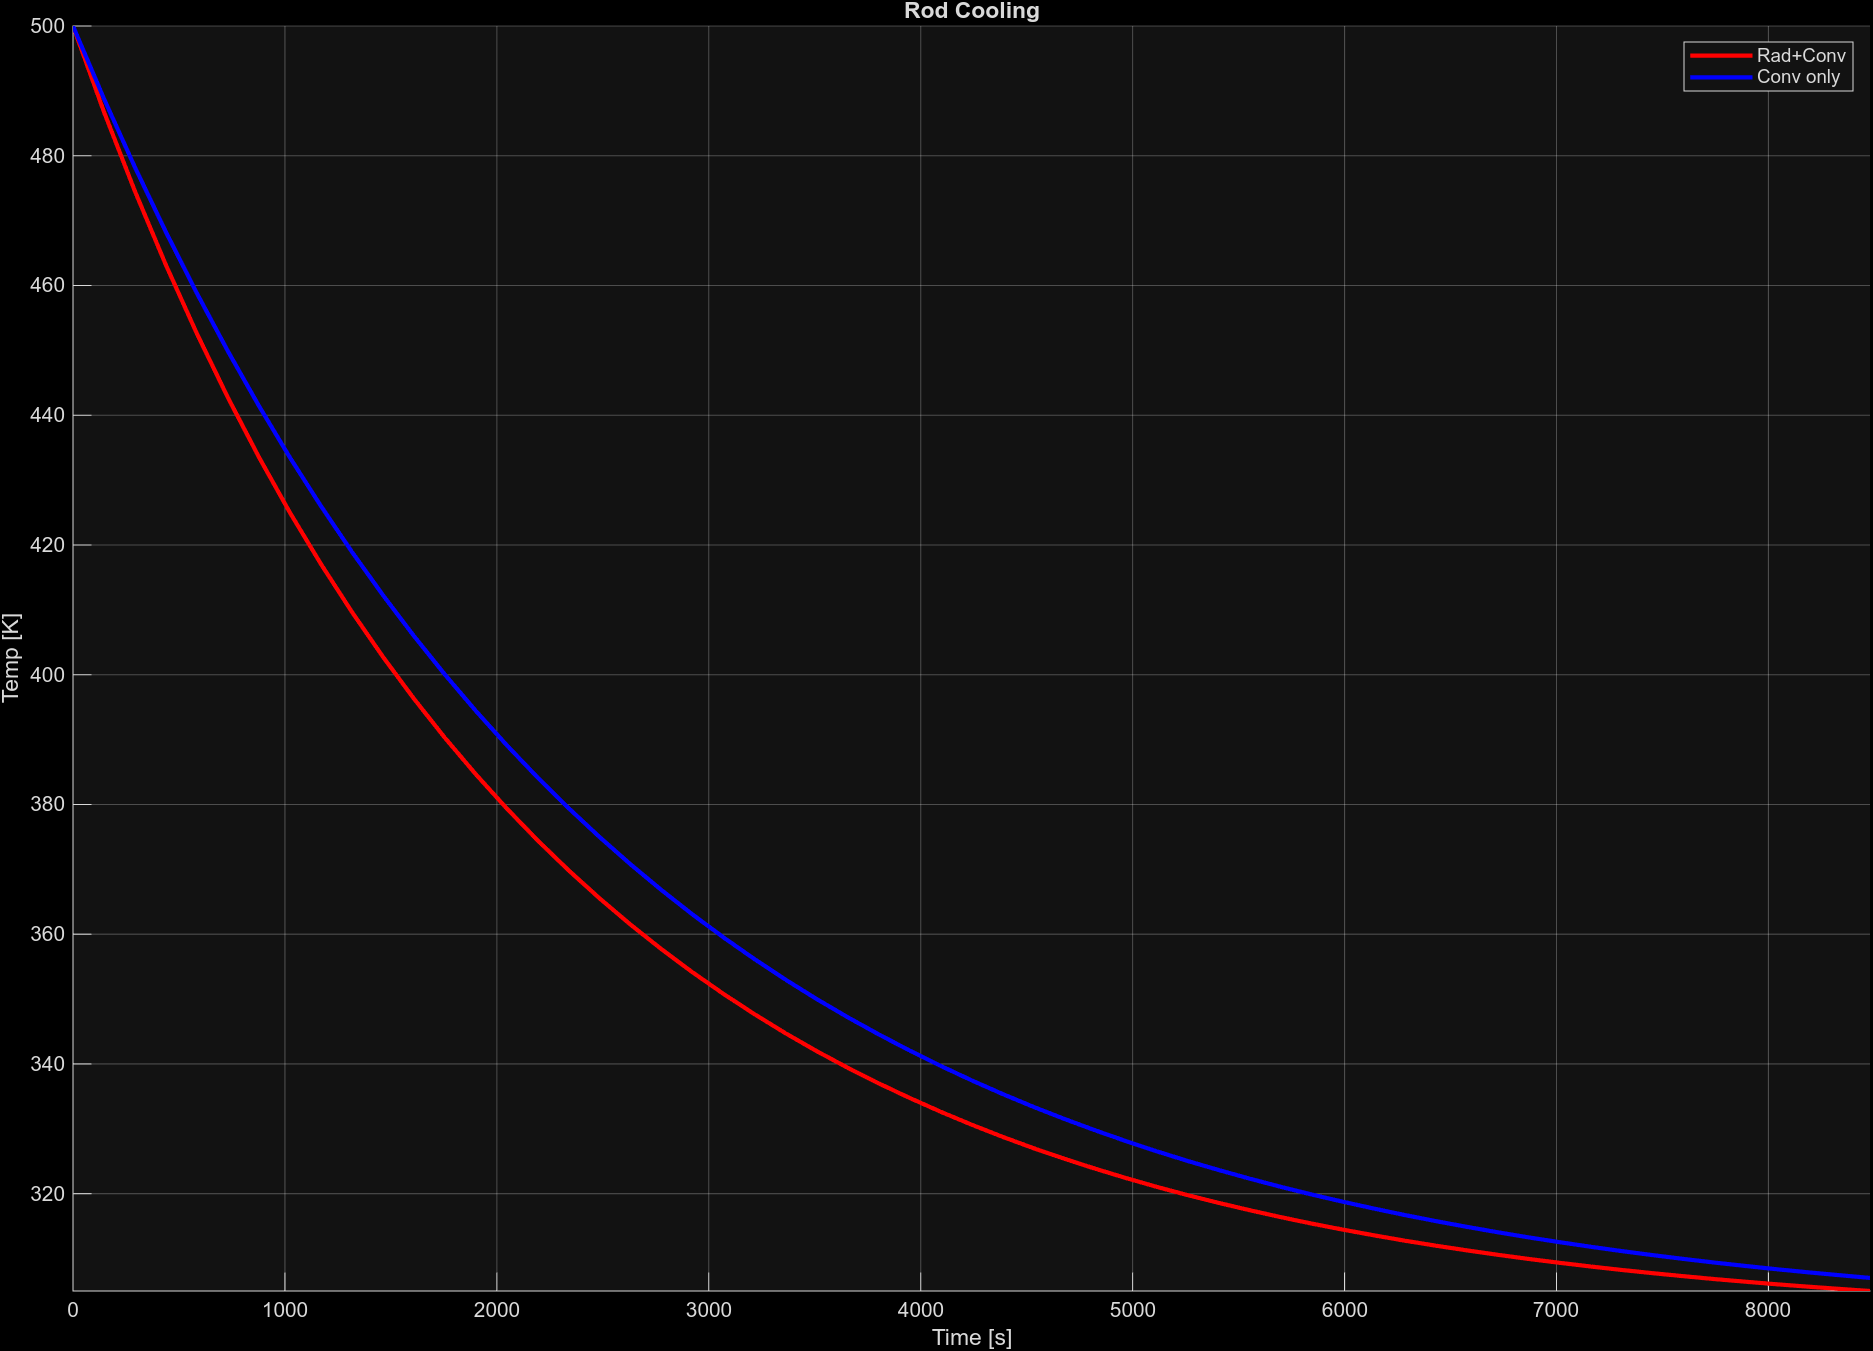
\includegraphics[width=0.7\textwidth]{/home/marian/myproject/Convection_Radiation/results/WithRadiation.png}
\caption{Temperature vs time for convection + radiation (\(\epsilon = 0.5\)).}
\label{fig:init}
\end{figure}

\begin{figure}[H]
\centering
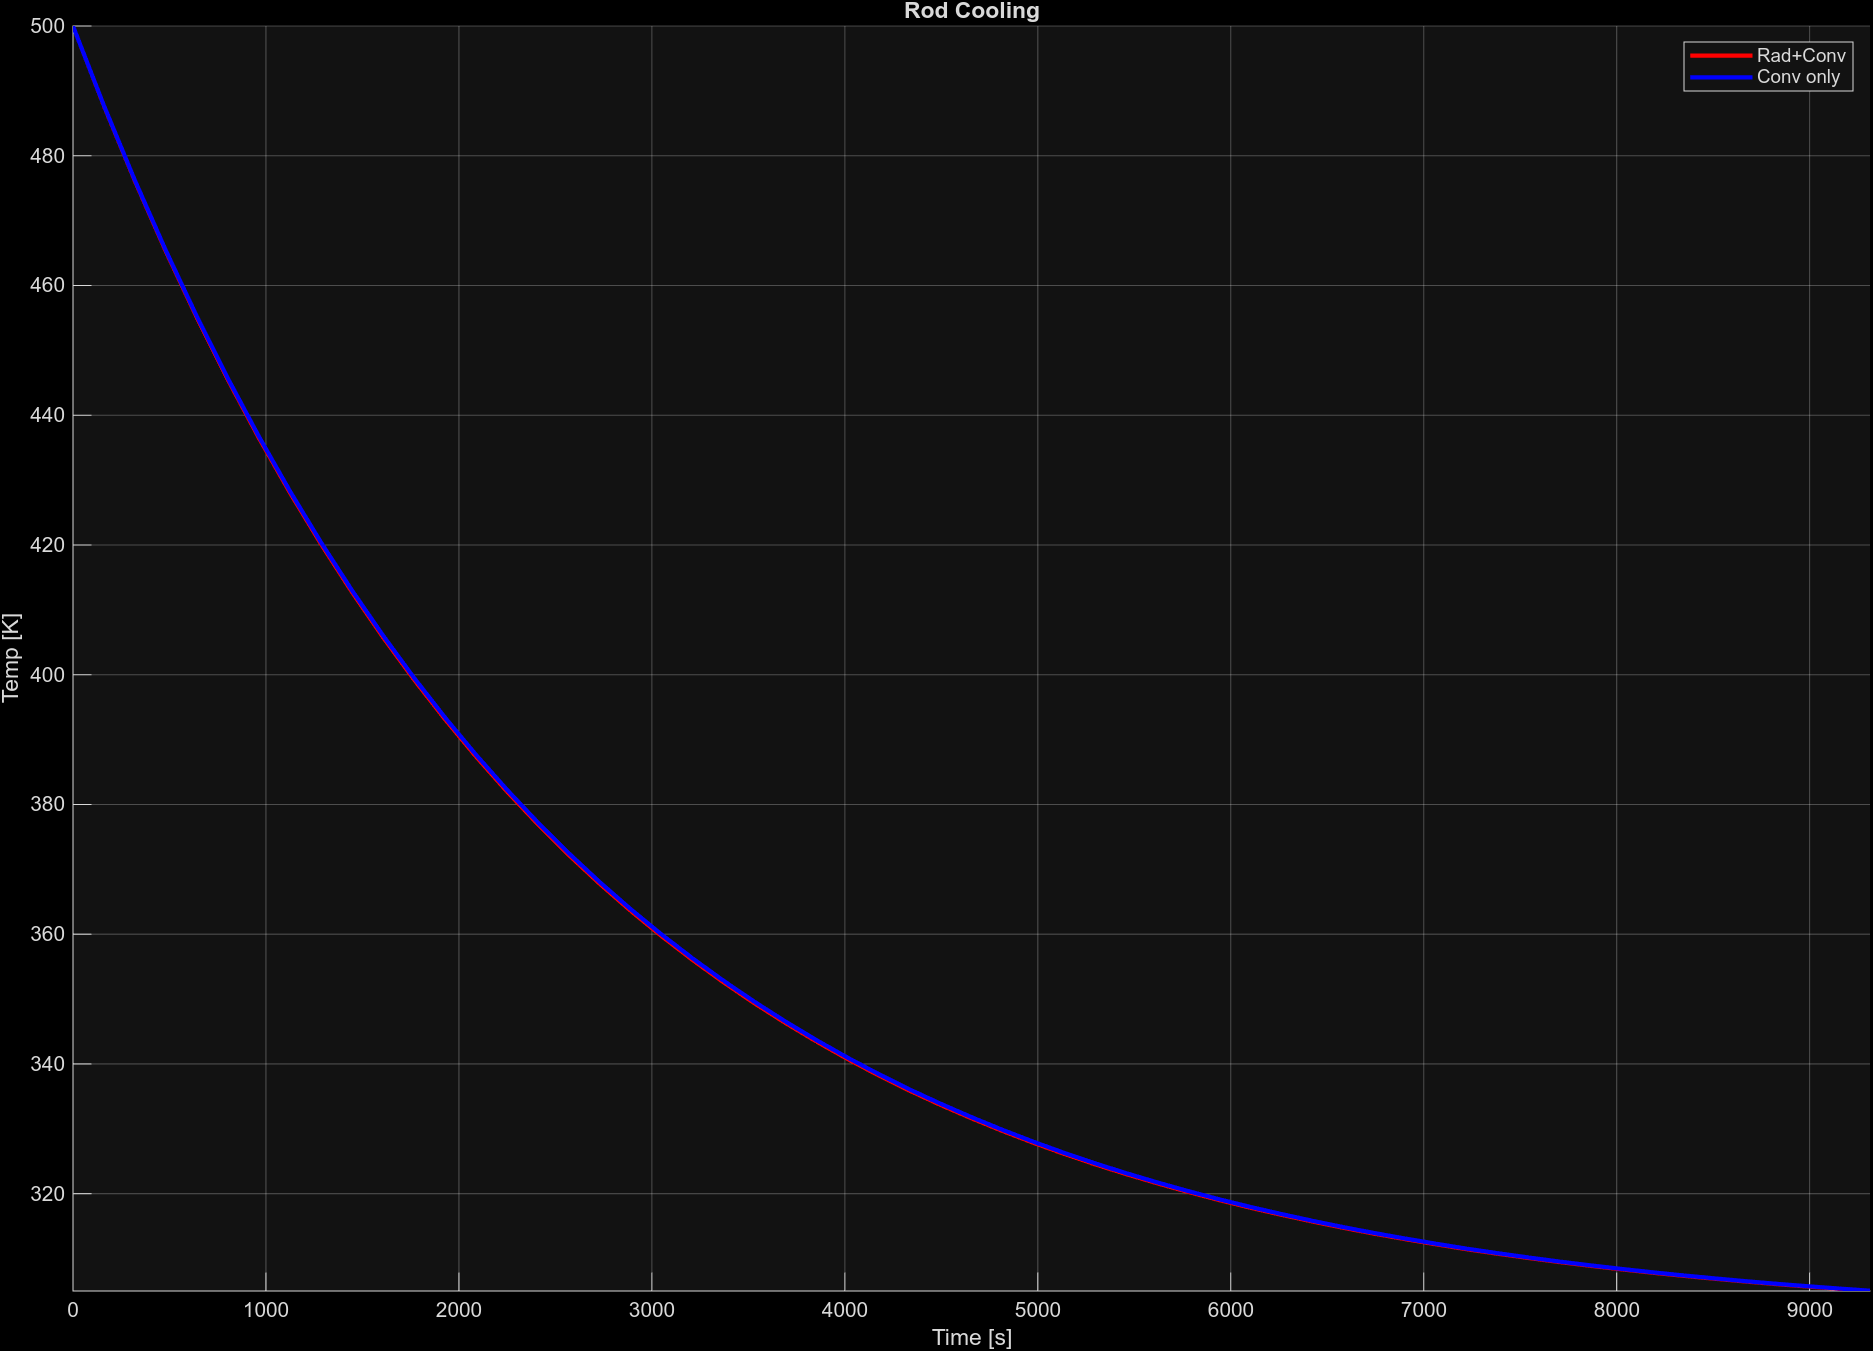
\includegraphics[width=0.7\textwidth]{/home/marian/myproject/Convection_Radiation/results/WithoutRadiation.png}
\caption{Temperature vs time with radiation disabled (\(\epsilon = 0\)), identical to convection-only solution.}
\label{fig:eps0}
\end{figure}

\section{Discussion}
\begin{itemize}
\item \textbf{Neglecting conduction:} The computed Biot number (\(\text{Bi} \approx 0.009 \ll 0.1\)) validates the lumped capacitance assumption.
\item \textbf{Effect of parameters:} Increasing \(T_0\) or \(h\) accelerates cooling. Emissivity (\(\epsilon\)) contributes significantly only at high temperatures or large differences from ambient.
\item \textbf{Visualization:} 3D cylinder animations with the \texttt{jet} colormap provide intuitive visual feedback of cooling dynamics.
\item \textbf{Validation:} Comparison between numerical solution and analytical convection-only solution shows good agreement.
\end{itemize}

\section{Conclusion}
The MATLAB simulation successfully demonstrates rod cooling under combined convection and radiation. The study confirms theoretical expectations, justifies the lumped capacitance approximation for low Biot numbers using a real material example, and provides an intuitive visual understanding of heat transfer dynamics.

\section{References}
\begin{enumerate}
\item Incropera, F.P., DeWitt, D.P., Bergman, T.L., Lavine, A.S., \textit{Fundamentals of Heat and Mass Transfer}, 7th Edition, Wiley, 2011.
\item MATLAB Documentation, \url{https://www.mathworks.com/help/matlab/}
\end{enumerate}

\end{document}
